\documentclass{article}

\usepackage[utf8]{inputenc}
\usepackage[french]{babel}

\usepackage{lmodern}
\usepackage{listings}
\usepackage{graphicx}
\usepackage{hyperref}
\usepackage{graphicx}
\usepackage{natbib}
\usepackage{tcolorbox}
\usepackage{xcolor}
\usepackage{array}
\usepackage{pifont}
\usepackage[a4paper, margin=1.5cm]{geometry}  
\usepackage{longtable}
\usepackage{float}
\usepackage{placeins}

\graphicspath{ {./res/} }
\author{
    Valentin Jonquière,
    Mathilde Chollon
}

\title{Rapport Architecture Logicielle}

\begin{document}

\maketitle

\pagebreak

\tableofcontents

\pagebreak

\section{Présentation du projet}

Ce rapport présente le projet du cours d'Architecture Logicielle de M1 Informatique à l'Université de Bordeaux.
Nous devions créer un logiciel de dessin vectoriel, où l'on peut manipuler différentes formes afin de créer des figures dans l'éditeur.
Le but de ce cours étant l'application de Design Patterns afin d'avoir une architecture propre, extensible et facilement maintenable, 
nous allons expliquer en section \ref{sec2} les patterns utilisés et leurs avantages pour notre implémentation.

Pour l'interface graphique, seulement quelques fonctions de \textit{Java AWT} étaient autorisées, comme les fonctions de dessin de rectangle, d'ovale ou de polygone, mais les types de formes devaient
être les nôtres.
Le logiciel présente plusieurs fonctionnalités clé qui sont les suivantes :
\begin{itemize}
    \item Sélection d'un objet depuis la toolbar et ajout au canevas via un glisser-déposer.
    \item Création/ suppression de groupes d'objets.
    \item Modification de la taille, position, couleur,... des objets.
    \item Ajout des formes crées à la toolbar via glisser-déposer.
    \item Annuler/ refaire une action.
    \item Sauvegarde/chargement d'un fichier contenant canevas et toolbar.
    \item Sauvegarde de la toolbar en quittant le logiciel, recharge au de celle ci au lancement.
\end{itemize}

\begin{figure}[H]
    \centering
    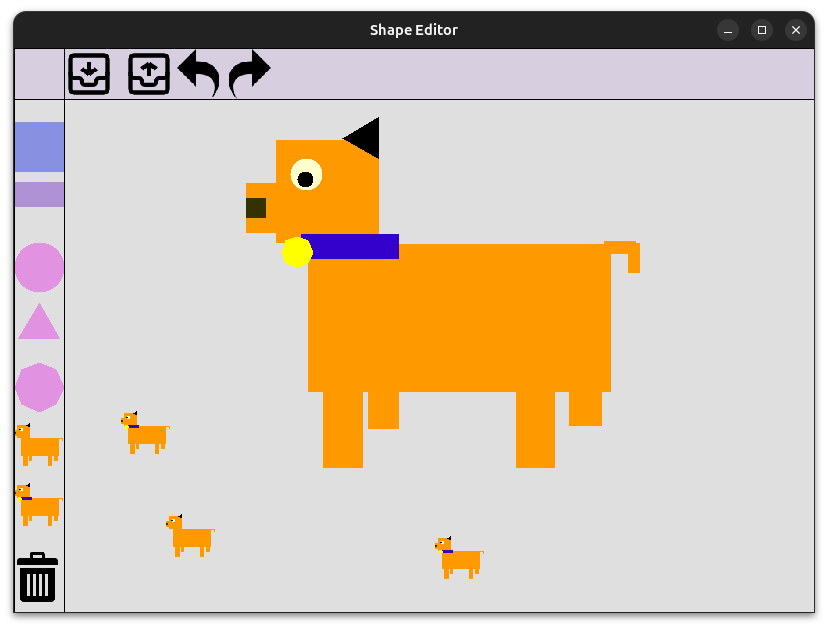
\includegraphics[width=0.8\textwidth,keepaspectratio]{dog.png}
    \caption{Exemple de dessin avec notre logiciel}
    \label{Clebs}
\end{figure}
\FloatBarrier
Sur la Figure \ref{Clebs}, on a un aperçu des différentes fonctionnalités du logiciel.
 Le chien a été créé à partir des formes basiques telles que le cercle, rectangle et polygone régulier.
 Grâce aux différentes possibilités d'édition de formes, nous avons pu changer la couleur, la forme ainsi que la tailles des formes pour créer le dessin voulu.
 On peut également voir que la forme a été ajoutée à la toolbar, et qu'il est possible de rajouter les formes de celles-ci au canevas.
 
\section{Design patterns utilisés} \label{sec2}

\subsection{Prototype}

\subsection{Builder}

\subsection{Composite}

\begin{figure}[h]
    \centering
    \includegraphics[width=\textwidth,height=20.0cm,keepaspectratio]{Composite.png}
    \caption{Diagramme UML du Composite}
    \label{Composite}
\end{figure}

\subsection{Singleton}

\subsection{Visitor}

\subsection{Method factory}

\subsection{Bridge}

\subsection{Observer}

\subsection{Bag Of Command}

\subsection{Memento}
\end{document}